\chapter{现有压缩感知缺陷检测原型分析}

目前,英国国家物理实验室 (NPL) 团队和西安电子科技大学团队分别独立完成了
基于压缩感知的太阳能电池缺陷检测装置原型。本章讨论这两套装置的设计和实现,
说明压缩感知方法在实际应用时遇到的一些问题。

\section{NPL 的原型装置}

NPL 自 2014 年起开始构建其基于压缩感知的太阳能缺陷检测装置原型。该装置的
光源为一激光二极管,其产生的 $636.2 nm$ 激光照射在一数字微镜器件 (DMD)
上。DMD 光学面上的大量微小镜面由外部提供的信号驱动,产生对应的结构光。
为了消除 DMD 产生的衍射效应,采用空间频率滤波器过滤结构光,
用过滤后的结构光照射被测太阳能电池。产生的光电流经 I-V
变换和采样后得到一次测量的结果。图 \ref{fig:npl} 给出 NPL 原型装置的框图。

\begin{figure}
\centering
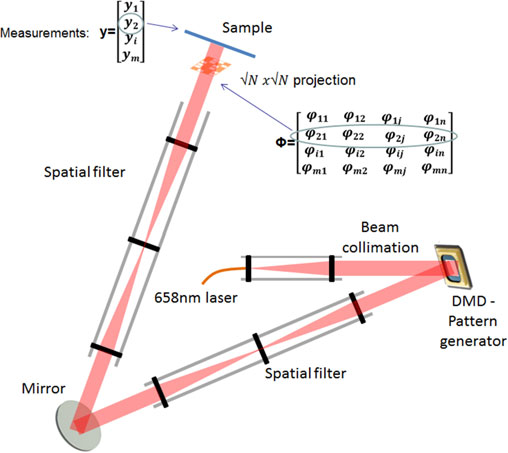
\includegraphics[width=.6\textwidth]{Figure/npl.png}
\caption{NPL 原型装置的原理图}
\label{fig:npl}
\end{figure}

NPL 装置采用一种称为 SBHE 的测量矩阵 \cite{BlockHadamard} :
\begin{definition}[SBHE 矩阵]
\begin{equation}
\Phi = Q_M W P_N
\end{equation}
其中
\begin{equation}
W = diag\{W_B, W_B, \cdots, W_B\}
\end{equation}
$W_B$ 是 $B \times B$ 的 Hadamard 矩阵,$P_N$ 是一个随机的置换矩阵,
$Q_M$ 是一个随机的 $M \times N$ 矩阵,选取 $W P_N$ 的 $M$ 行。
\end{definition}

和完全随机的测量矩阵相比,SBHE 的突出优点是计算复杂度较小。置换
$P_N$ 只需要 $O(N)$ ,$Q_M$ 的作用是选取 $M$ 行,只需要 $O(M)$ ,而
$W$ 相当于 $N/B$ 次快速 Hadamard-Walsh 变换,时间复杂度为
\begin{equation}
T(N,B) = O(N + M + N/B \times B log B) = O(N(1+logB))
\end{equation}
相比于完全随机矩阵需要 $O(NM)$ 的运算时间,SBHE 的运算速度要快得多,可以
有效减少重建时间。和 Bernoulli 矩阵一样, SBHE 是二值化的,因此容易在光学
系统中实现。实践表明,一般选取 $B=32$ 就能得到较好的效果。

\section{西安电子科技大学的原型装置}

和 NPL 的实现相比,西安电子科技大学团队的原型装置是在较短时间内完成的,
其结构也较为简单。作为研究原型,它没有使用 DMD ,而是直接将待测太阳能电池
贴在 LCD 显示器上,由显示器提供结构光,如图 \ref{fig:xdu} 所示。
这种方法成本较低,但不能适用于更大
的太阳能组件。另外,由于没有使用激光光源,结构光的光谱并不匹配太阳能电池
的最大响应波段,这些问题需要在后续实验中进行改进。

\begin{figure}
\centering
\includegraphics[width=.6\textwidth]{Figure/xdu.pdf}
\caption{(a) LCD 显示的随机模式。 (b) 太阳能电池的感光面被贴在 LCD 表面,
其输出电流被测量。}
\label{fig:xdu}
\end{figure}

文献 \cite{XDUCLBIC} 指出,该装置相比于传统的 LBIC 扫描法,时间效率有
$10$ 至 $15$ 倍的提升。实际上,时间效率的提升是两种因素的共同作用。首先,
该装置使用 LCD 作为光源,避免了机械运动环节,极大地提升了测量效率。例如,
对于某一特定太阳能电池, LBIC 需要对 $6400$ 个测试点依次扫描,消耗时间为
$1280 s$ 左右。而 CLBIC 系统即使在测量 $6400$ 个光电流数据的情况下,测量
过程和图像重建过程的总时间
也仅有 $170 s$,相当于时间效率提高 $7$ 倍。其次,根据压缩感知理论, CLBIC
系统对光电流的测量次数比 LBIC 少。例如,如果将测量次数减少到测试点个数的
$30\%$ ,即 $1920$ 次,则 CLBIC 的总耗时进一步减小到 $87 s$ ,时间效率相比
进行 $6400$ 次采样时又提升 $1$ 倍,相比于 LBIC 方法提升 $15$ 倍。

理论上,我们当然可以用 LCD 代替机械扫描装置,在每次测量时只点亮 LCD 的一个
测试点,从而直接得到太阳能电池的缺陷分布。然而,实际上,由于没有聚焦装置,
这种方法浪费了 LCD 光源的绝大多数能量,导致信噪比大幅下降,实践中根本不足
取。而压缩感知方法则不然,在压缩感知的测量中,每次均有约一半的光源能量被
利用。因此,尽管 LCD 引起的效率提升看上去和压缩感知无关,实际上却只有压缩
感知方法才能直接使用 LCD 作为光源,从而避免聚焦和机械扫描。

\section{原型装置遇到的问题}

在实验过程中,两个原型装置遇到了一些共同的问题。

(1) 太阳能电池的栅状电极破坏了测量结果的稀疏性,正如在仿真中发现的一样,
栅状电极的存在导致我们要增加 $20\%$ 至 $40\%$ 的测量,提高了测量和恢复需要
的时间。

(2) 在采样次数接近 $90\%$ 的时候,从理论上讲,应该得到非常好的恢复结果。
然而,两个团队都发现,由于噪声的存在,当采样次数较大时,根本无法得到有意义
的恢复结果。进一步的分析表明,造成这一现象的噪声作用于测量矩阵,而非采样
结果本身,压缩感知恢复算法的抗噪能力对矩阵噪声不能发挥作用。

(3) 随着问题规模的提高,恢复算法的运算量以立方级别增加。如果要在工业上
使用压缩感知方法检测太阳能缺陷,势必遇到运算量过大的问题。对此,两个团队
都建议,可以使用云计算、 FPGA 等高并发的编程平台来缓解这一问题,并应对
恢复算法进行改进和优化,以减小计算量。
